\documentclass[11pt]{article}
\usepackage[textwidth=18.0cm, textheight=23.0cm, top=2.0cm]{geometry}
\usepackage{pst-all}
\usepackage{amssymb}
\usepackage{tikz}
\usepackage{underscore}\begin{document}
\pagestyle{empty}


ClassName: \underline{\textbf{Class_08.2bp-20}}
\par
BinSize: \underline{\textbf{100 × 100}}
\par
ReduceSize: \underline{\textbf{100 × 100}}
\par
TypeNum: \underline{\textbf{60}}
\par
Num: \underline{\textbf{60}}
\par
OutS: \underline{\textbf{170000}}
\par
InS: \underline{\textbf{145807}}
\par
Rate: \underline{\textbf{0.858}}
\par
UB: \underline{\textbf{17}}
\par
LB0: \underline{\textbf{17}}
\par
LB: \underline{\textbf{17}}
\par
LBWithCut: \underline{\textbf{17}}
\par
NodeCut: \underline{\textbf{0}}
\par
ExtendedNodeCnt: \underline{\textbf{1}}
\par
GenNodeCnt: \underline{\textbf{1}}
\par
PrimalNode: \underline{\textbf{0}}
\par
ColumnCount: \underline{\textbf{17}}
\par
TotalCutCount: \underline{\textbf{0}}
\par
RootCutCount: \underline{\textbf{0}}
\par
LPSolverCnt: \underline{\textbf{1}}
\par
PricingSolverCnt: \underline{\textbf{0}}
\par
BranchAndBoundNum: \underline{\textbf{1}}
\par
isOpt: \underline{\textbf{true}}
\par
TimeOnInitSolution: \underline{\textbf{0.090 s}}
\par
TimeOnPrimal: \underline{\textbf{0.000 s}}
\par
TimeOnPricing: \underline{\textbf{0.000 s}}
\par
TimeOnRmp: \underline{\textbf{0.093 s}}
\par
TotalTime: \underline{\textbf{0.262 s}}
\par
\newpage


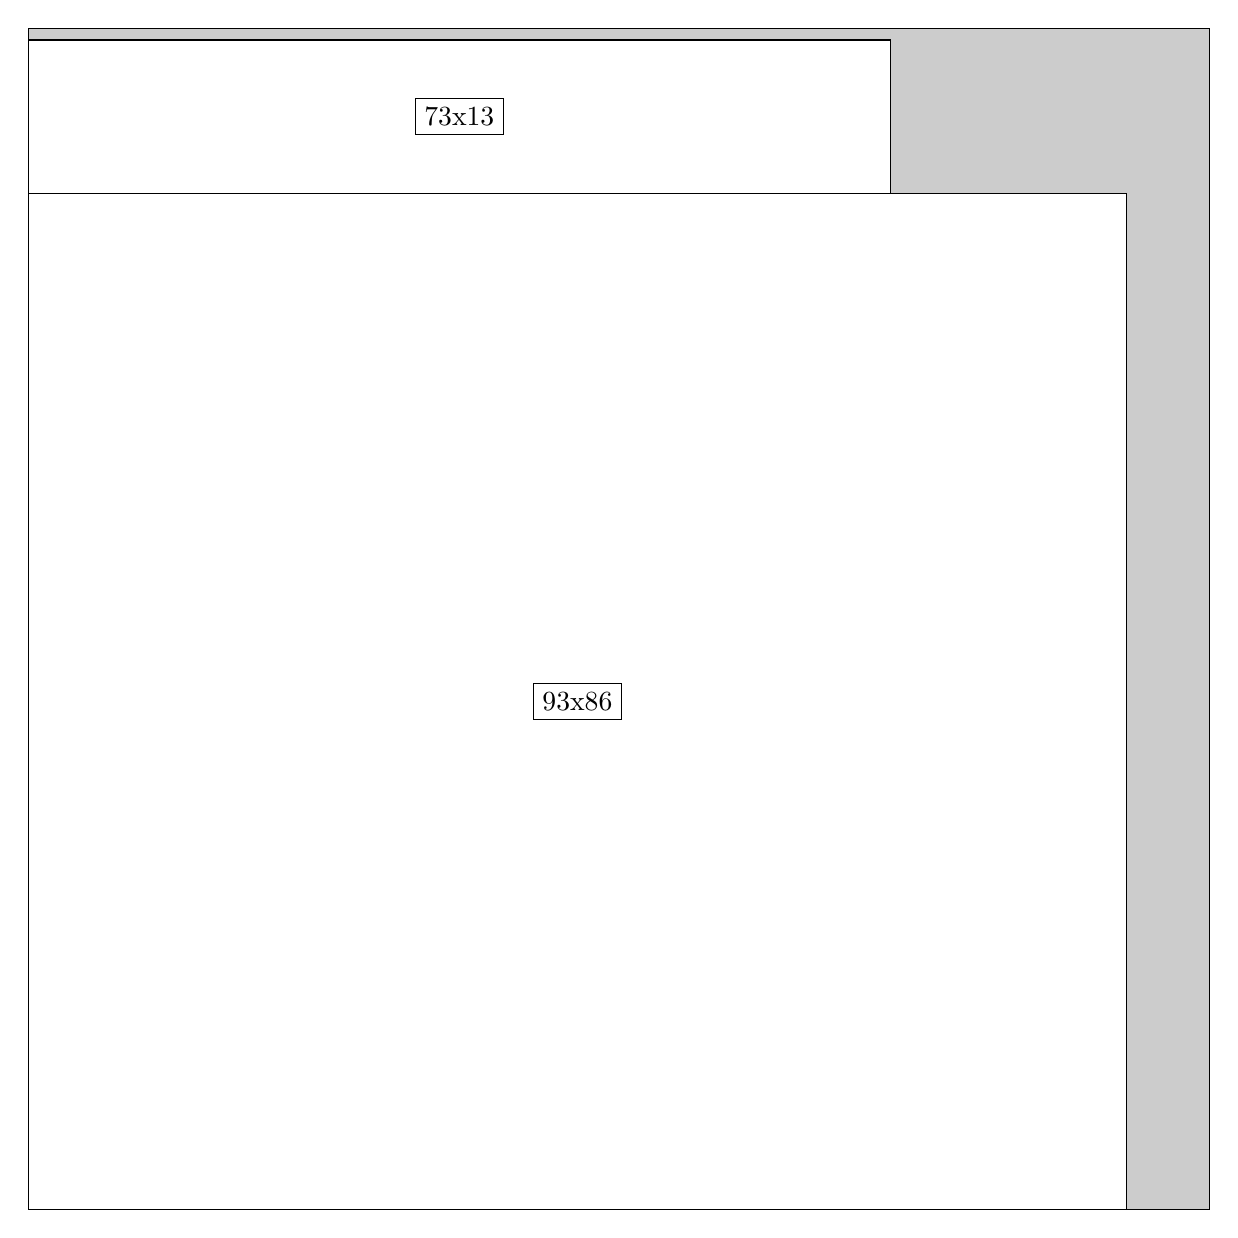
\begin{tikzpicture}[shorten >=1pt,scale=1.0,every node/.style={scale=1.0},->]
\tikzstyle{vertex}=[circle,fill=black!25,minimum size=14pt,inner sep=0pt]
\filldraw[fill=gray!40!white, draw=black] (0,0) rectangle (15.0,15.0);
\foreach \name/\x/\y/\w/\h in {93x86/0.0/0.0/13.95/12.9,73x13/0.0/12.9/10.95/1.95}
\filldraw[fill=white!40!white, draw=black] (\x,\y) rectangle node[draw] (\name) {\name} ++(\w,\h);
\end{tikzpicture}


w =93 , h =86 , x =0 , y =0 , v =7998
\par
w =73 , h =13 , x =0 , y =86 , v =949
\par
\newpage


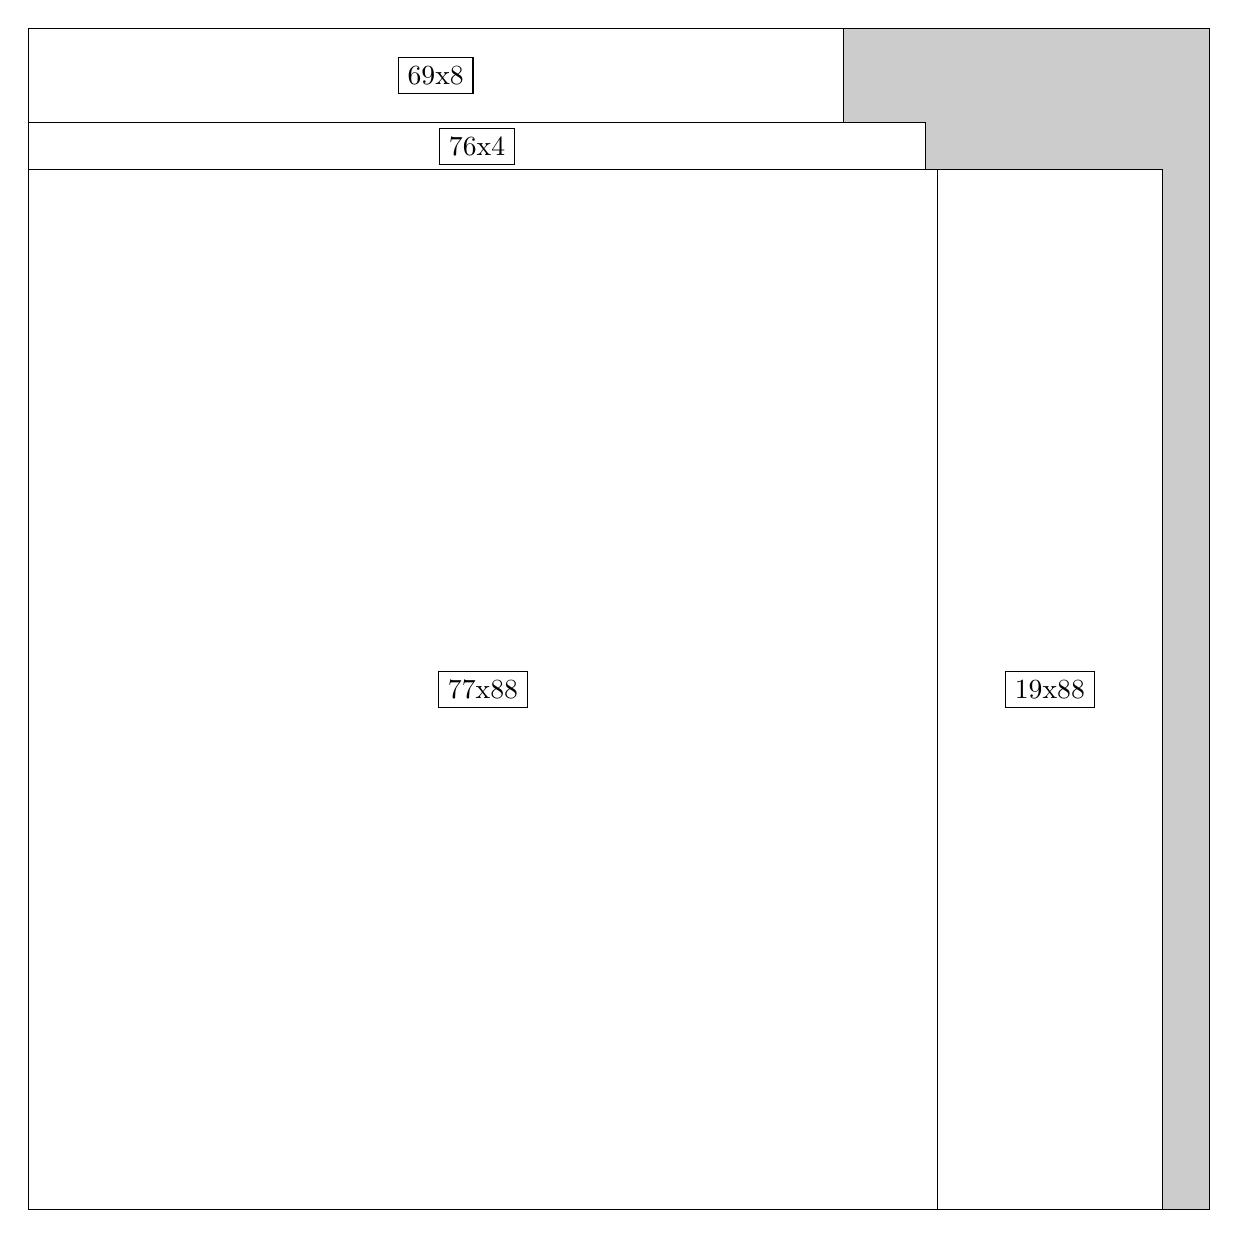
\begin{tikzpicture}[shorten >=1pt,scale=1.0,every node/.style={scale=1.0},->]
\tikzstyle{vertex}=[circle,fill=black!25,minimum size=14pt,inner sep=0pt]
\filldraw[fill=gray!40!white, draw=black] (0,0) rectangle (15.0,15.0);
\foreach \name/\x/\y/\w/\h in {77x88/0.0/0.0/11.549999999999999/13.2,19x88/11.549999999999999/0.0/2.85/13.2,69x8/0.0/13.799999999999999/10.35/1.2,76x4/0.0/13.2/11.4/0.6}
\filldraw[fill=white!40!white, draw=black] (\x,\y) rectangle node[draw] (\name) {\name} ++(\w,\h);
\end{tikzpicture}


w =77 , h =88 , x =0 , y =0 , v =6776
\par
w =19 , h =88 , x =77 , y =0 , v =1672
\par
w =69 , h =8 , x =0 , y =92 , v =552
\par
w =76 , h =4 , x =0 , y =88 , v =304
\par
\newpage


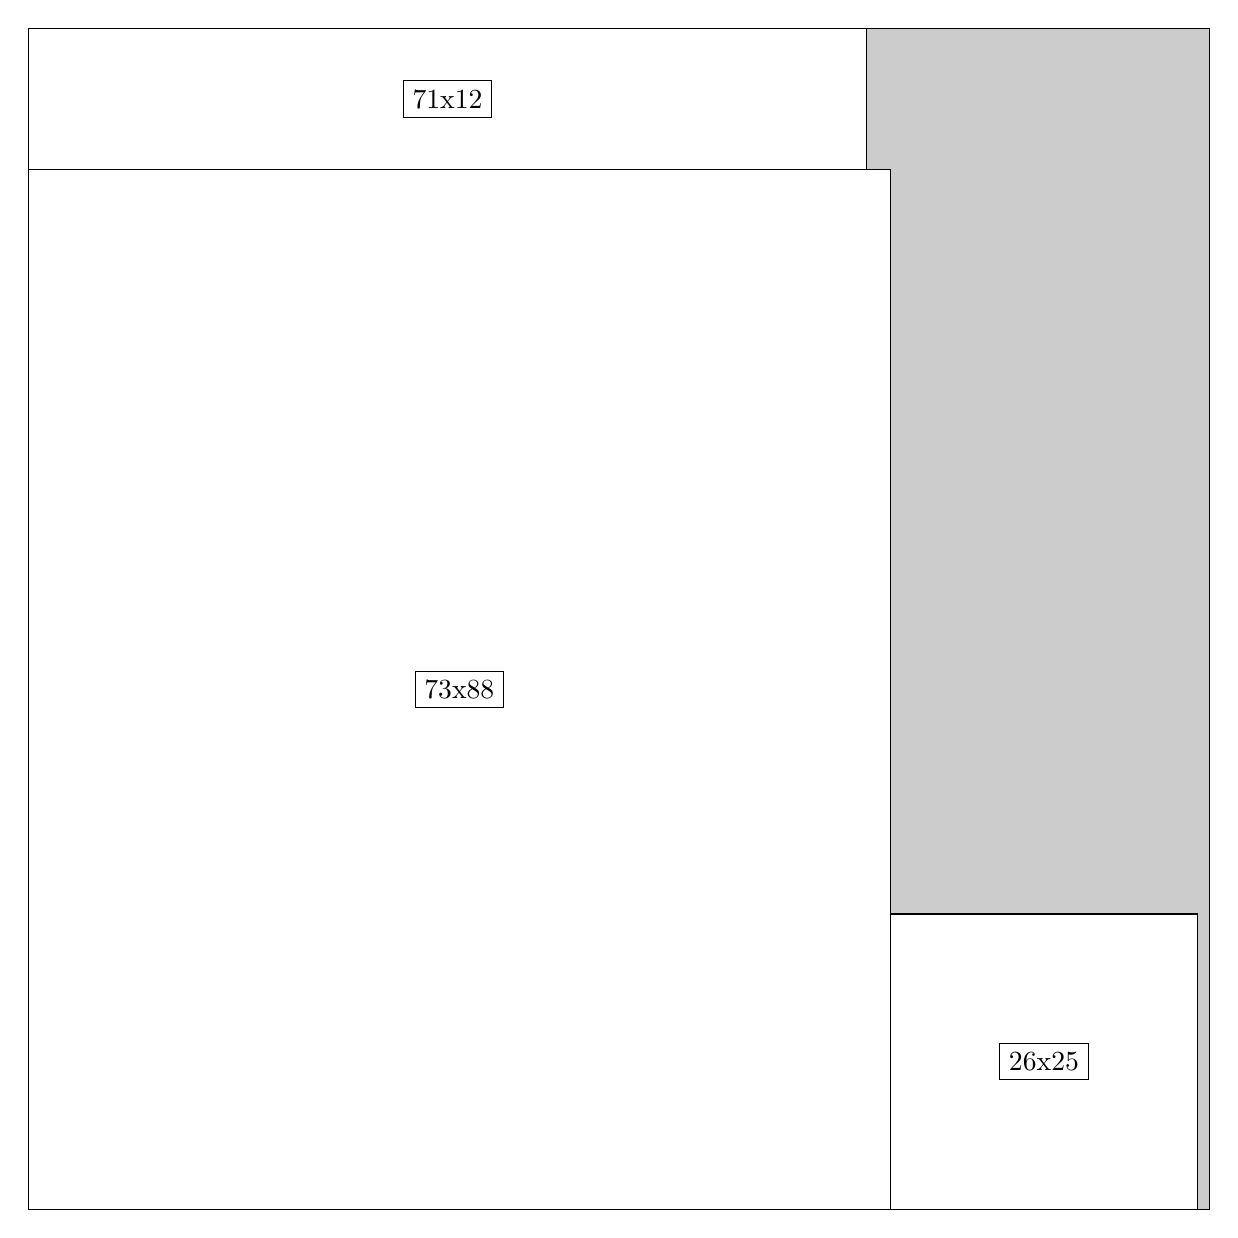
\begin{tikzpicture}[shorten >=1pt,scale=1.0,every node/.style={scale=1.0},->]
\tikzstyle{vertex}=[circle,fill=black!25,minimum size=14pt,inner sep=0pt]
\filldraw[fill=gray!40!white, draw=black] (0,0) rectangle (15.0,15.0);
\foreach \name/\x/\y/\w/\h in {73x88/0.0/0.0/10.95/13.2,71x12/0.0/13.2/10.65/1.7999999999999998,26x25/10.95/0.0/3.9/3.75}
\filldraw[fill=white!40!white, draw=black] (\x,\y) rectangle node[draw] (\name) {\name} ++(\w,\h);
\end{tikzpicture}


w =73 , h =88 , x =0 , y =0 , v =6424
\par
w =71 , h =12 , x =0 , y =88 , v =852
\par
w =26 , h =25 , x =73 , y =0 , v =650
\par
\newpage


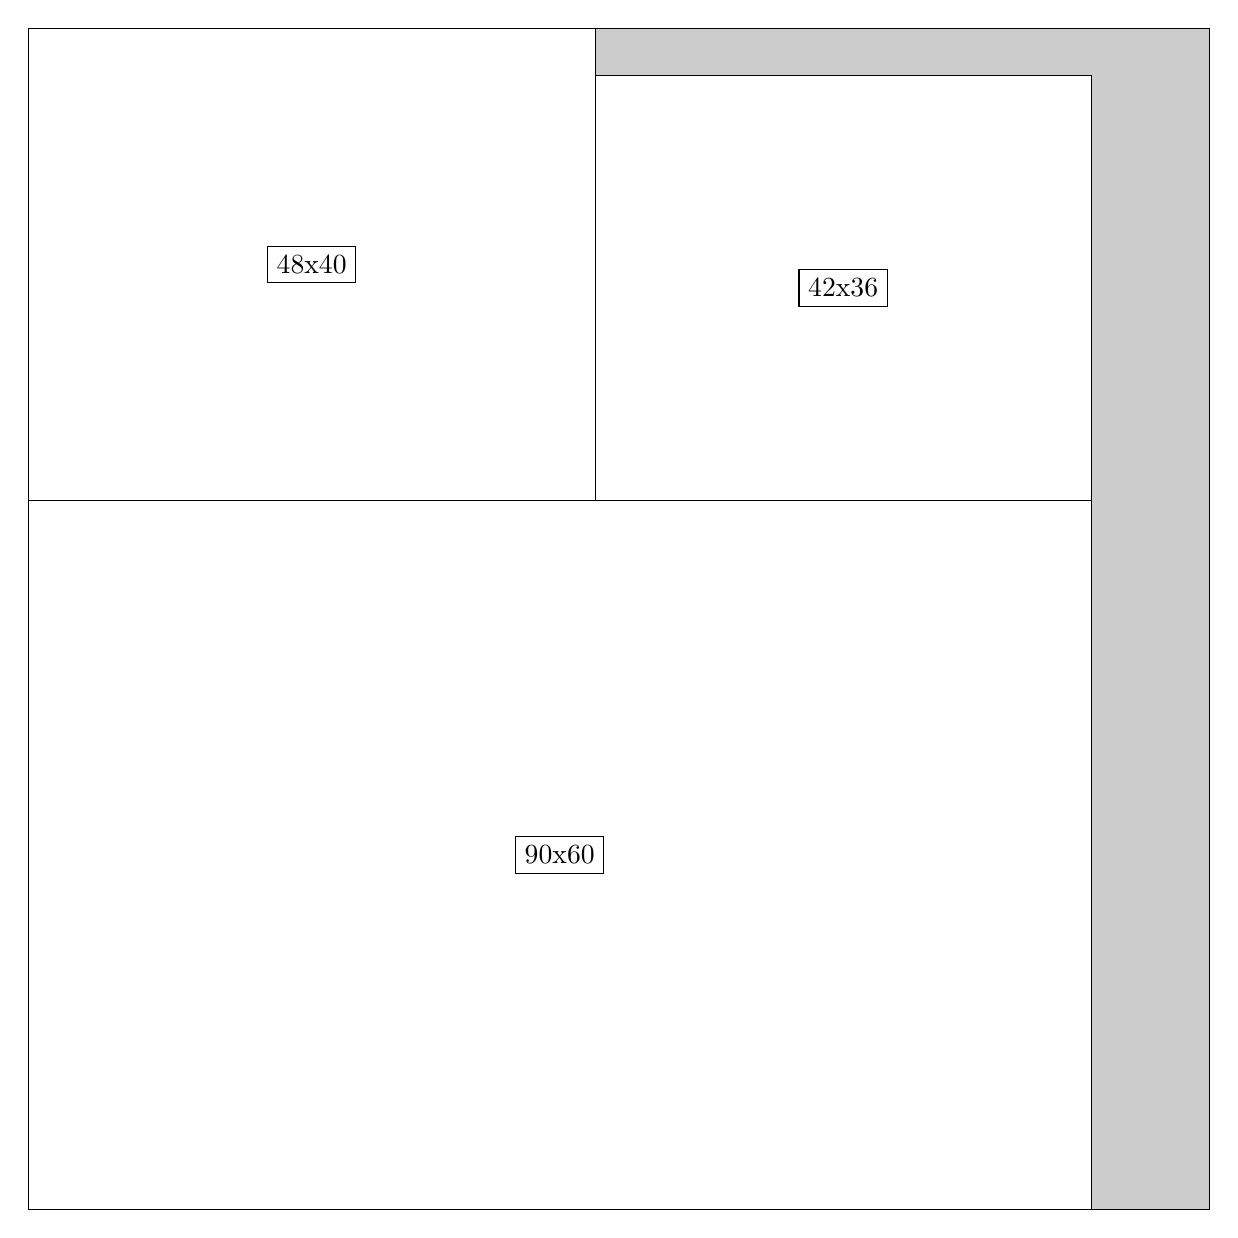
\begin{tikzpicture}[shorten >=1pt,scale=1.0,every node/.style={scale=1.0},->]
\tikzstyle{vertex}=[circle,fill=black!25,minimum size=14pt,inner sep=0pt]
\filldraw[fill=gray!40!white, draw=black] (0,0) rectangle (15.0,15.0);
\foreach \name/\x/\y/\w/\h in {90x60/0.0/0.0/13.5/9.0,48x40/0.0/9.0/7.199999999999999/6.0,42x36/7.199999999999999/9.0/6.3/5.3999999999999995}
\filldraw[fill=white!40!white, draw=black] (\x,\y) rectangle node[draw] (\name) {\name} ++(\w,\h);
\end{tikzpicture}


w =90 , h =60 , x =0 , y =0 , v =5400
\par
w =48 , h =40 , x =0 , y =60 , v =1920
\par
w =42 , h =36 , x =48 , y =60 , v =1512
\par
\newpage


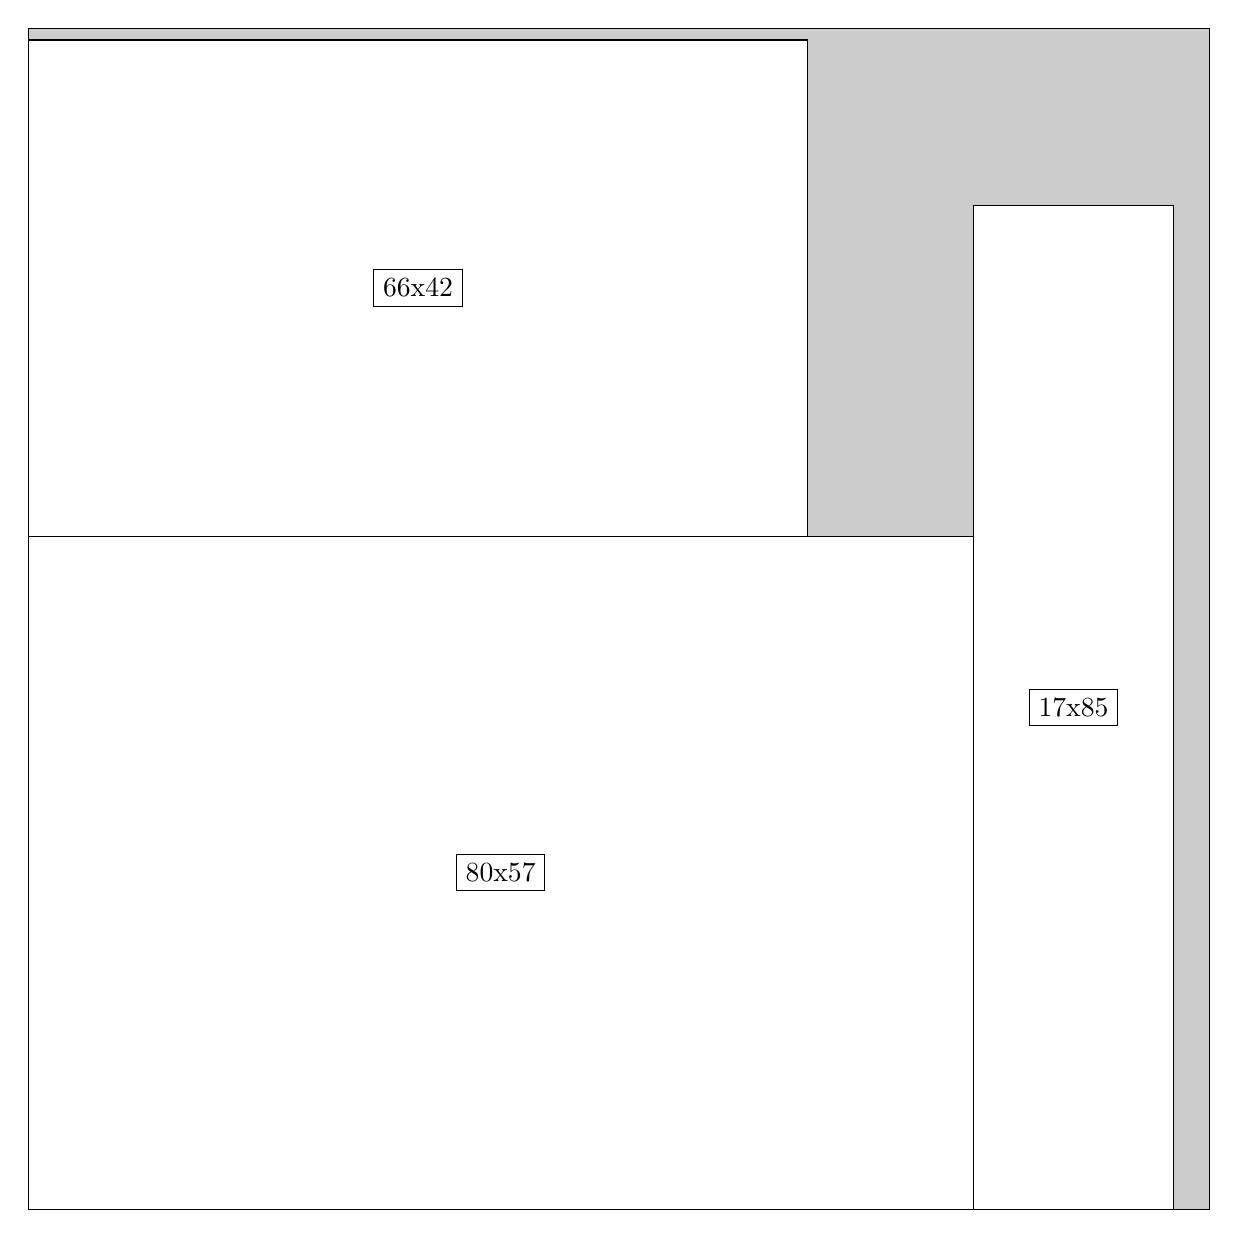
\begin{tikzpicture}[shorten >=1pt,scale=1.0,every node/.style={scale=1.0},->]
\tikzstyle{vertex}=[circle,fill=black!25,minimum size=14pt,inner sep=0pt]
\filldraw[fill=gray!40!white, draw=black] (0,0) rectangle (15.0,15.0);
\foreach \name/\x/\y/\w/\h in {80x57/0.0/0.0/12.0/8.549999999999999,66x42/0.0/8.549999999999999/9.9/6.3,17x85/12.0/0.0/2.55/12.75}
\filldraw[fill=white!40!white, draw=black] (\x,\y) rectangle node[draw] (\name) {\name} ++(\w,\h);
\end{tikzpicture}


w =80 , h =57 , x =0 , y =0 , v =4560
\par
w =66 , h =42 , x =0 , y =57 , v =2772
\par
w =17 , h =85 , x =80 , y =0 , v =1445
\par
\newpage


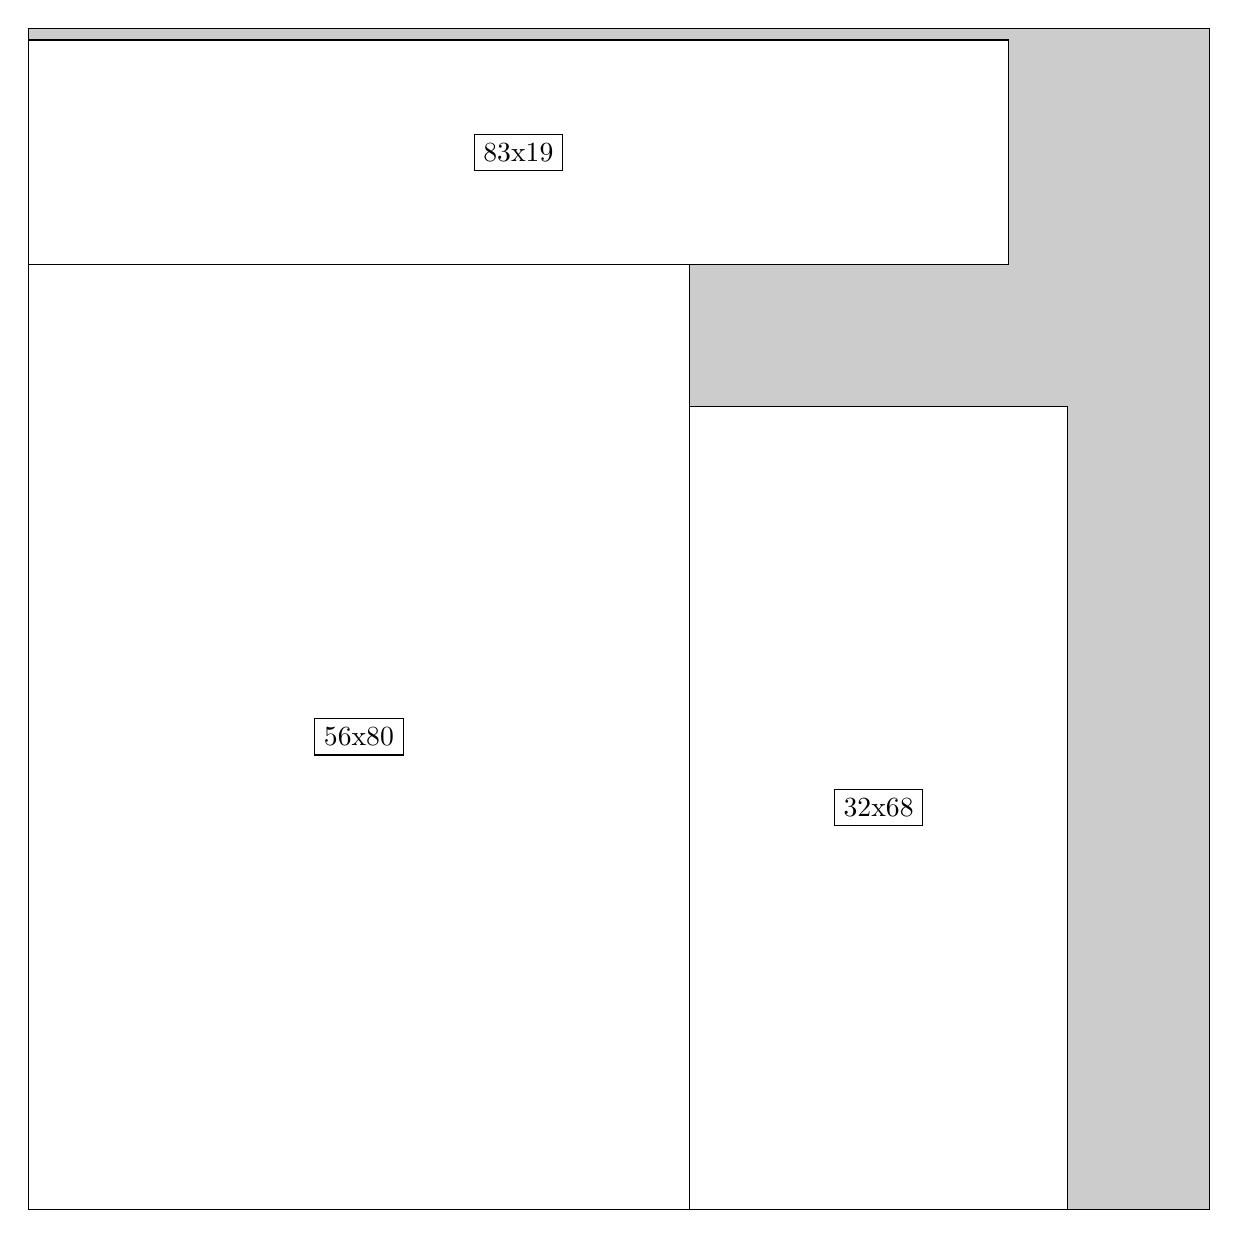
\begin{tikzpicture}[shorten >=1pt,scale=1.0,every node/.style={scale=1.0},->]
\tikzstyle{vertex}=[circle,fill=black!25,minimum size=14pt,inner sep=0pt]
\filldraw[fill=gray!40!white, draw=black] (0,0) rectangle (15.0,15.0);
\foreach \name/\x/\y/\w/\h in {56x80/0.0/0.0/8.4/12.0,32x68/8.4/0.0/4.8/10.2,83x19/0.0/12.0/12.45/2.85}
\filldraw[fill=white!40!white, draw=black] (\x,\y) rectangle node[draw] (\name) {\name} ++(\w,\h);
\end{tikzpicture}


w =56 , h =80 , x =0 , y =0 , v =4480
\par
w =32 , h =68 , x =56 , y =0 , v =2176
\par
w =83 , h =19 , x =0 , y =80 , v =1577
\par
\newpage


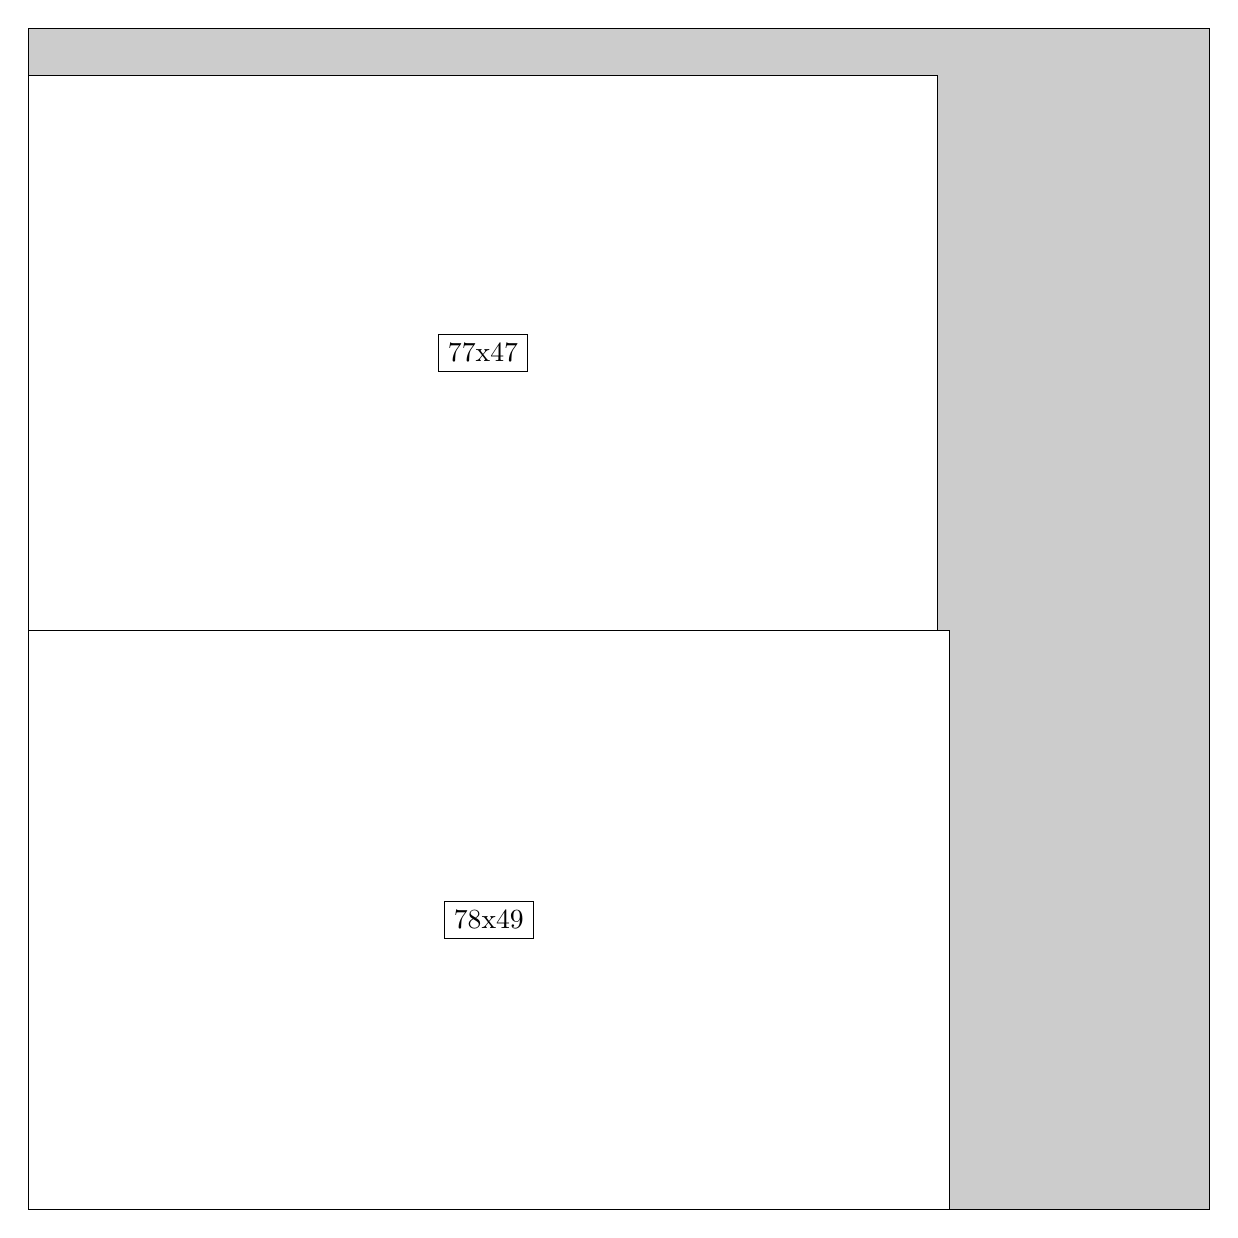
\begin{tikzpicture}[shorten >=1pt,scale=1.0,every node/.style={scale=1.0},->]
\tikzstyle{vertex}=[circle,fill=black!25,minimum size=14pt,inner sep=0pt]
\filldraw[fill=gray!40!white, draw=black] (0,0) rectangle (15.0,15.0);
\foreach \name/\x/\y/\w/\h in {78x49/0.0/0.0/11.7/7.35,77x47/0.0/7.35/11.549999999999999/7.05}
\filldraw[fill=white!40!white, draw=black] (\x,\y) rectangle node[draw] (\name) {\name} ++(\w,\h);
\end{tikzpicture}


w =78 , h =49 , x =0 , y =0 , v =3822
\par
w =77 , h =47 , x =0 , y =49 , v =3619
\par
\newpage


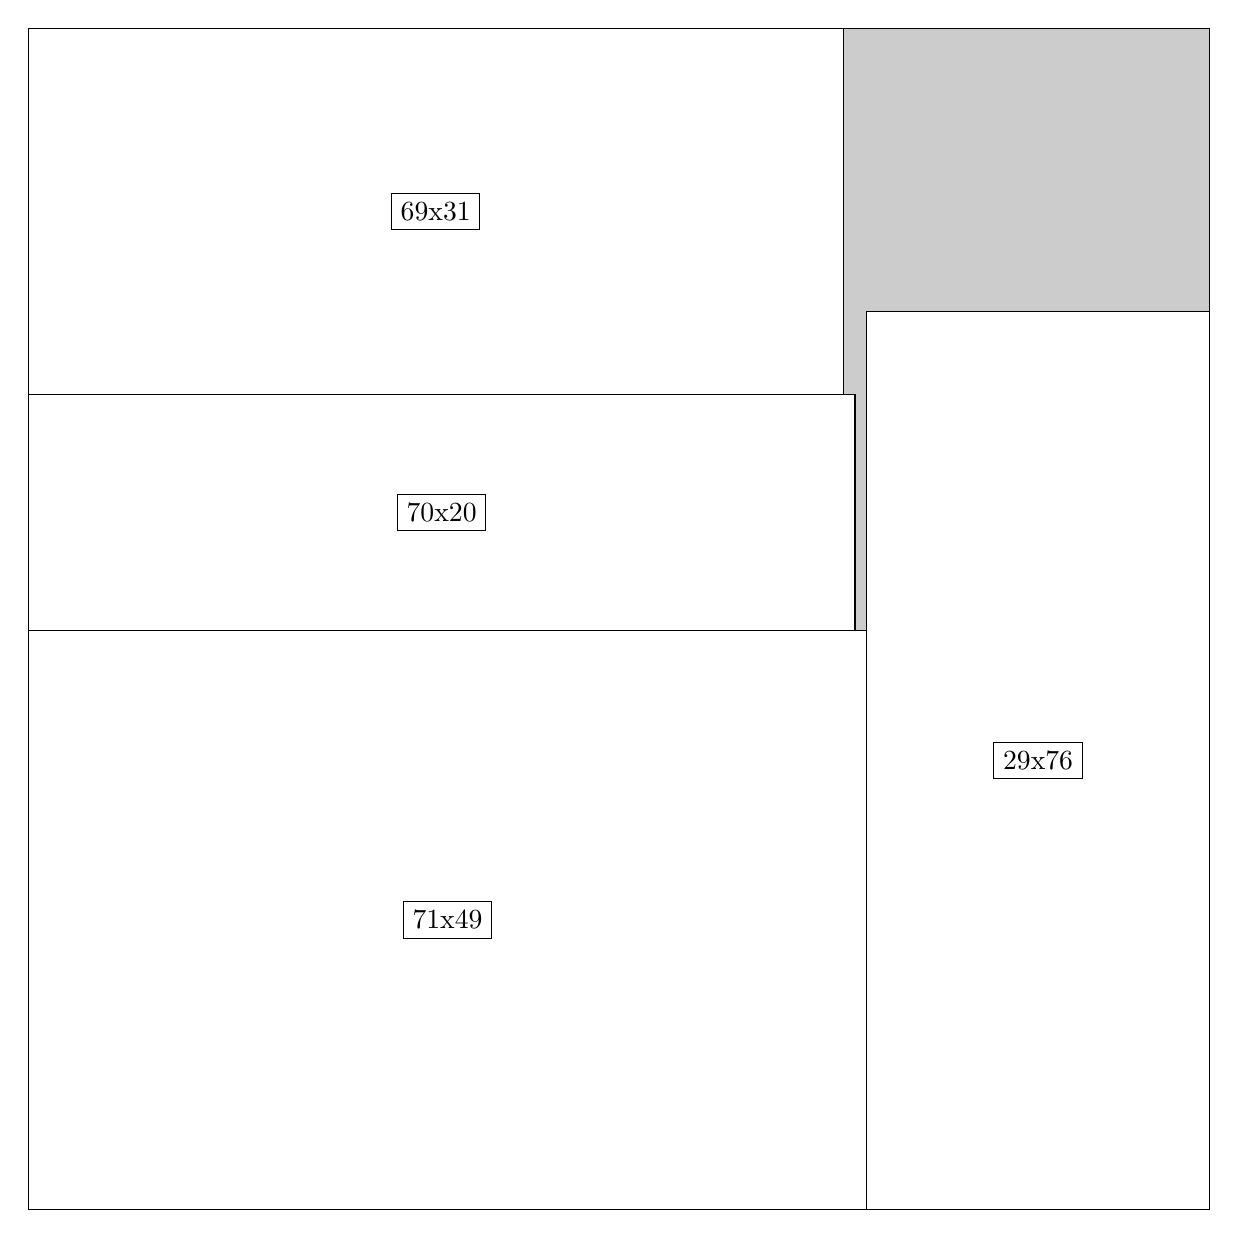
\begin{tikzpicture}[shorten >=1pt,scale=1.0,every node/.style={scale=1.0},->]
\tikzstyle{vertex}=[circle,fill=black!25,minimum size=14pt,inner sep=0pt]
\filldraw[fill=gray!40!white, draw=black] (0,0) rectangle (15.0,15.0);
\foreach \name/\x/\y/\w/\h in {71x49/0.0/0.0/10.65/7.35,29x76/10.65/0.0/4.35/11.4,69x31/0.0/10.35/10.35/4.6499999999999995,70x20/0.0/7.35/10.5/3.0}
\filldraw[fill=white!40!white, draw=black] (\x,\y) rectangle node[draw] (\name) {\name} ++(\w,\h);
\end{tikzpicture}


w =71 , h =49 , x =0 , y =0 , v =3479
\par
w =29 , h =76 , x =71 , y =0 , v =2204
\par
w =69 , h =31 , x =0 , y =69 , v =2139
\par
w =70 , h =20 , x =0 , y =49 , v =1400
\par
\newpage


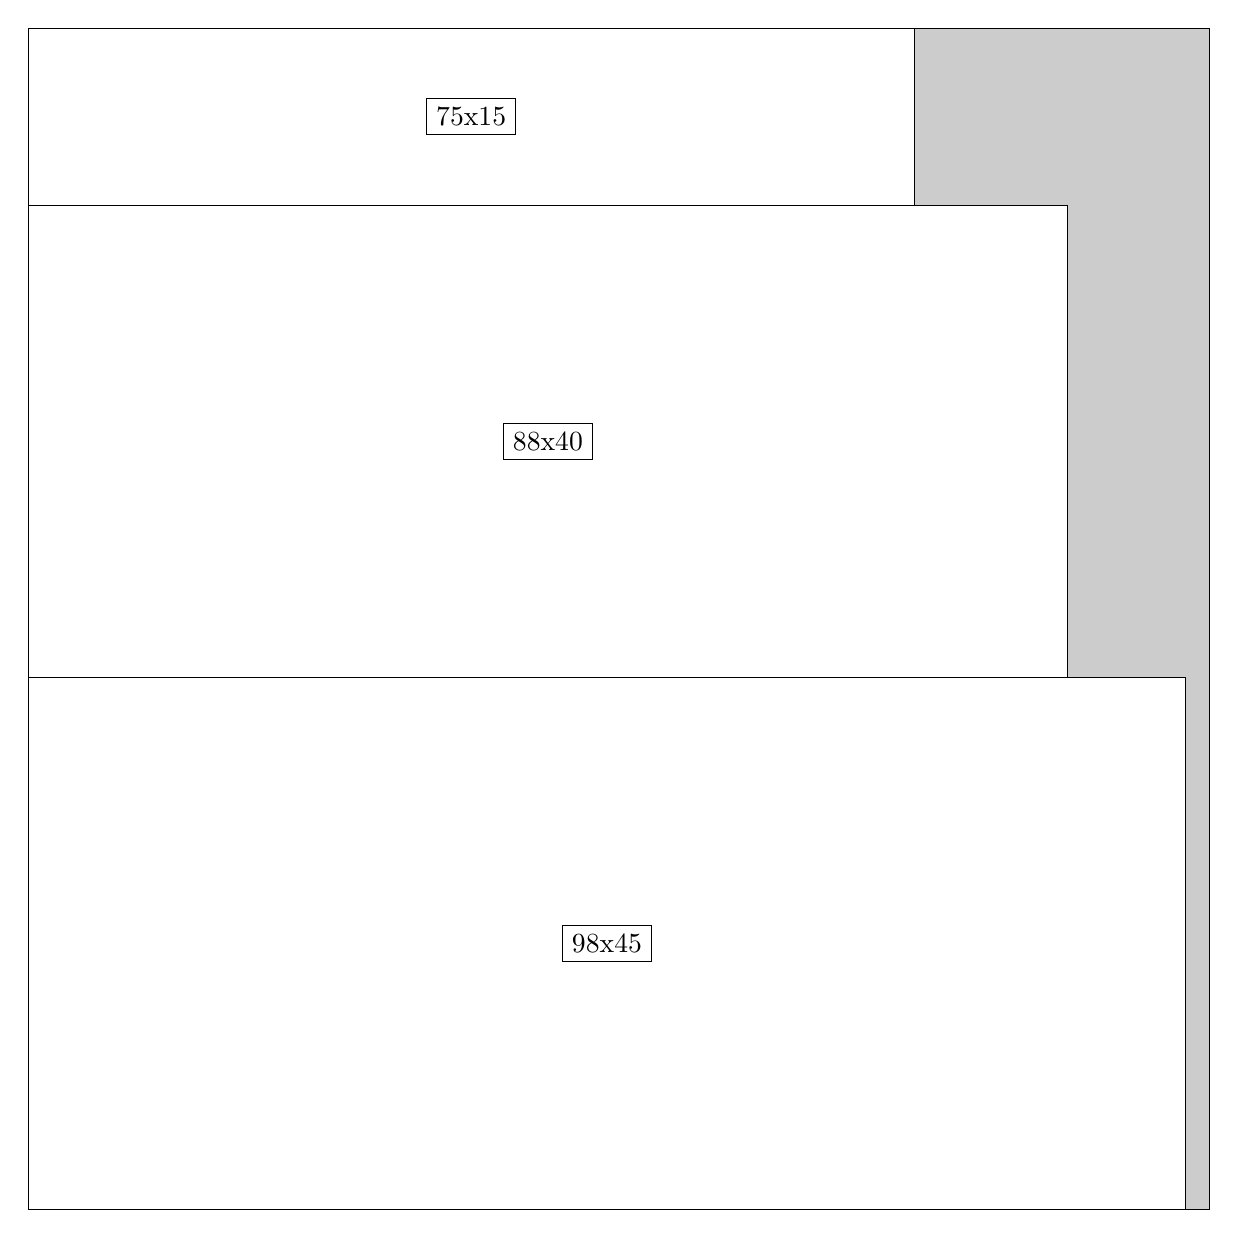
\begin{tikzpicture}[shorten >=1pt,scale=1.0,every node/.style={scale=1.0},->]
\tikzstyle{vertex}=[circle,fill=black!25,minimum size=14pt,inner sep=0pt]
\filldraw[fill=gray!40!white, draw=black] (0,0) rectangle (15.0,15.0);
\foreach \name/\x/\y/\w/\h in {98x45/0.0/0.0/14.7/6.75,88x40/0.0/6.75/13.2/6.0,75x15/0.0/12.75/11.25/2.25}
\filldraw[fill=white!40!white, draw=black] (\x,\y) rectangle node[draw] (\name) {\name} ++(\w,\h);
\end{tikzpicture}


w =98 , h =45 , x =0 , y =0 , v =4410
\par
w =88 , h =40 , x =0 , y =45 , v =3520
\par
w =75 , h =15 , x =0 , y =85 , v =1125
\par
\newpage


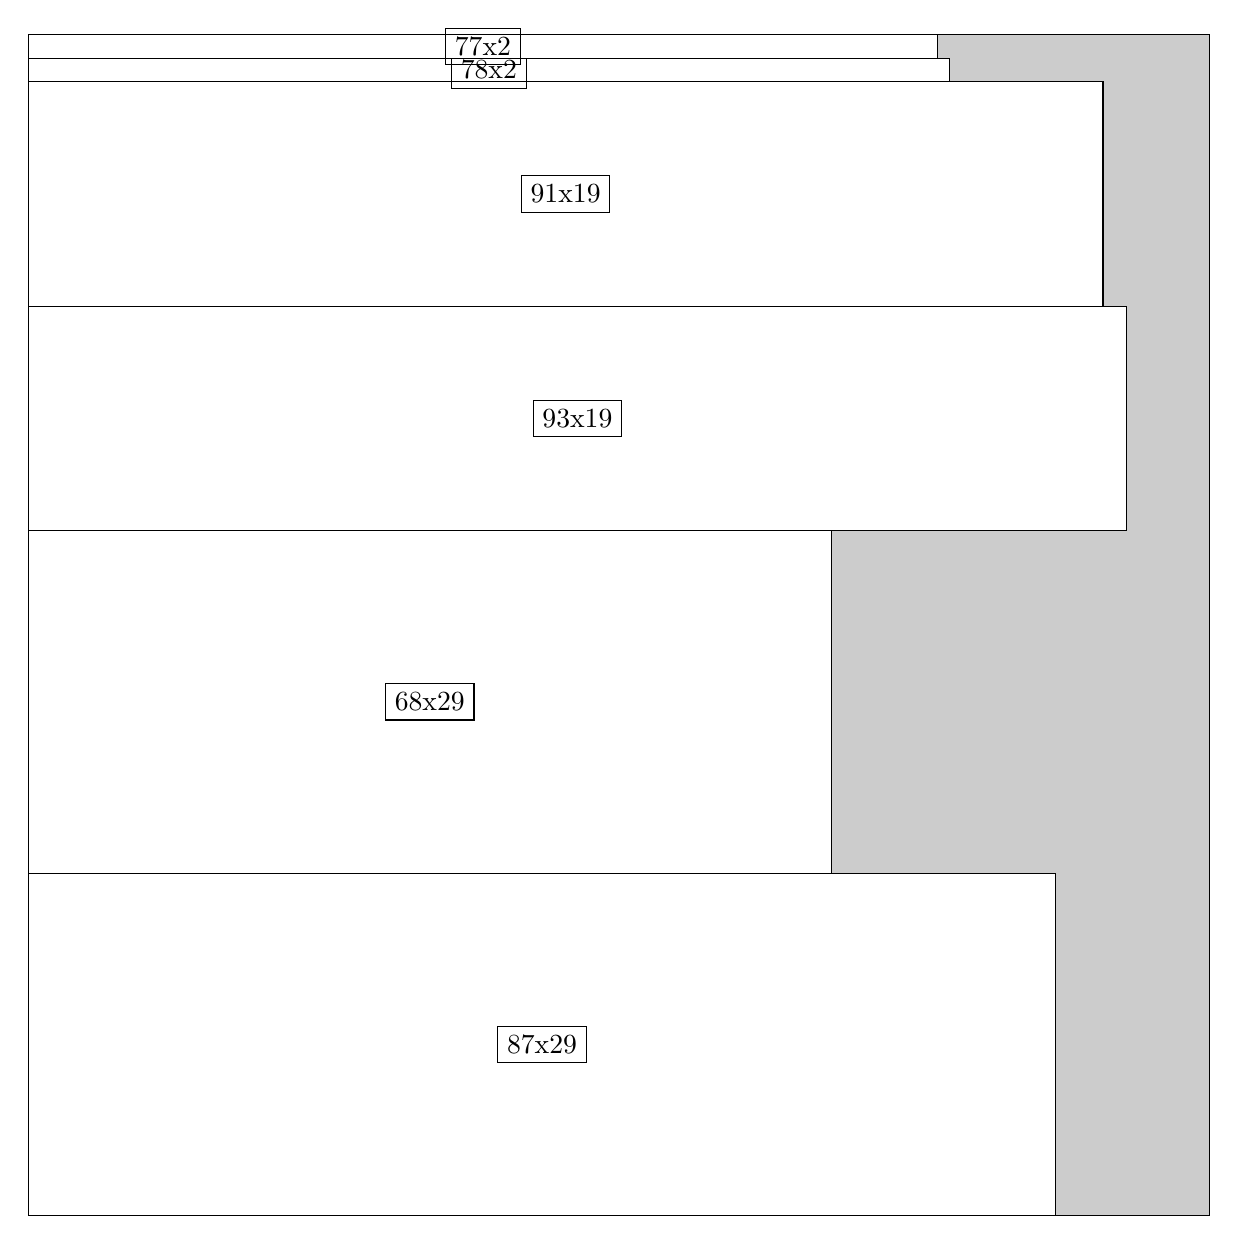
\begin{tikzpicture}[shorten >=1pt,scale=1.0,every node/.style={scale=1.0},->]
\tikzstyle{vertex}=[circle,fill=black!25,minimum size=14pt,inner sep=0pt]
\filldraw[fill=gray!40!white, draw=black] (0,0) rectangle (15.0,15.0);
\foreach \name/\x/\y/\w/\h in {87x29/0.0/0.0/13.049999999999999/4.35,68x29/0.0/4.35/10.2/4.35,93x19/0.0/8.7/13.95/2.85,91x19/0.0/11.549999999999999/13.65/2.85,78x2/0.0/14.399999999999999/11.7/0.3,77x2/0.0/14.7/11.549999999999999/0.3}
\filldraw[fill=white!40!white, draw=black] (\x,\y) rectangle node[draw] (\name) {\name} ++(\w,\h);
\end{tikzpicture}


w =87 , h =29 , x =0 , y =0 , v =2523
\par
w =68 , h =29 , x =0 , y =29 , v =1972
\par
w =93 , h =19 , x =0 , y =58 , v =1767
\par
w =91 , h =19 , x =0 , y =77 , v =1729
\par
w =78 , h =2 , x =0 , y =96 , v =156
\par
w =77 , h =2 , x =0 , y =98 , v =154
\par
\newpage


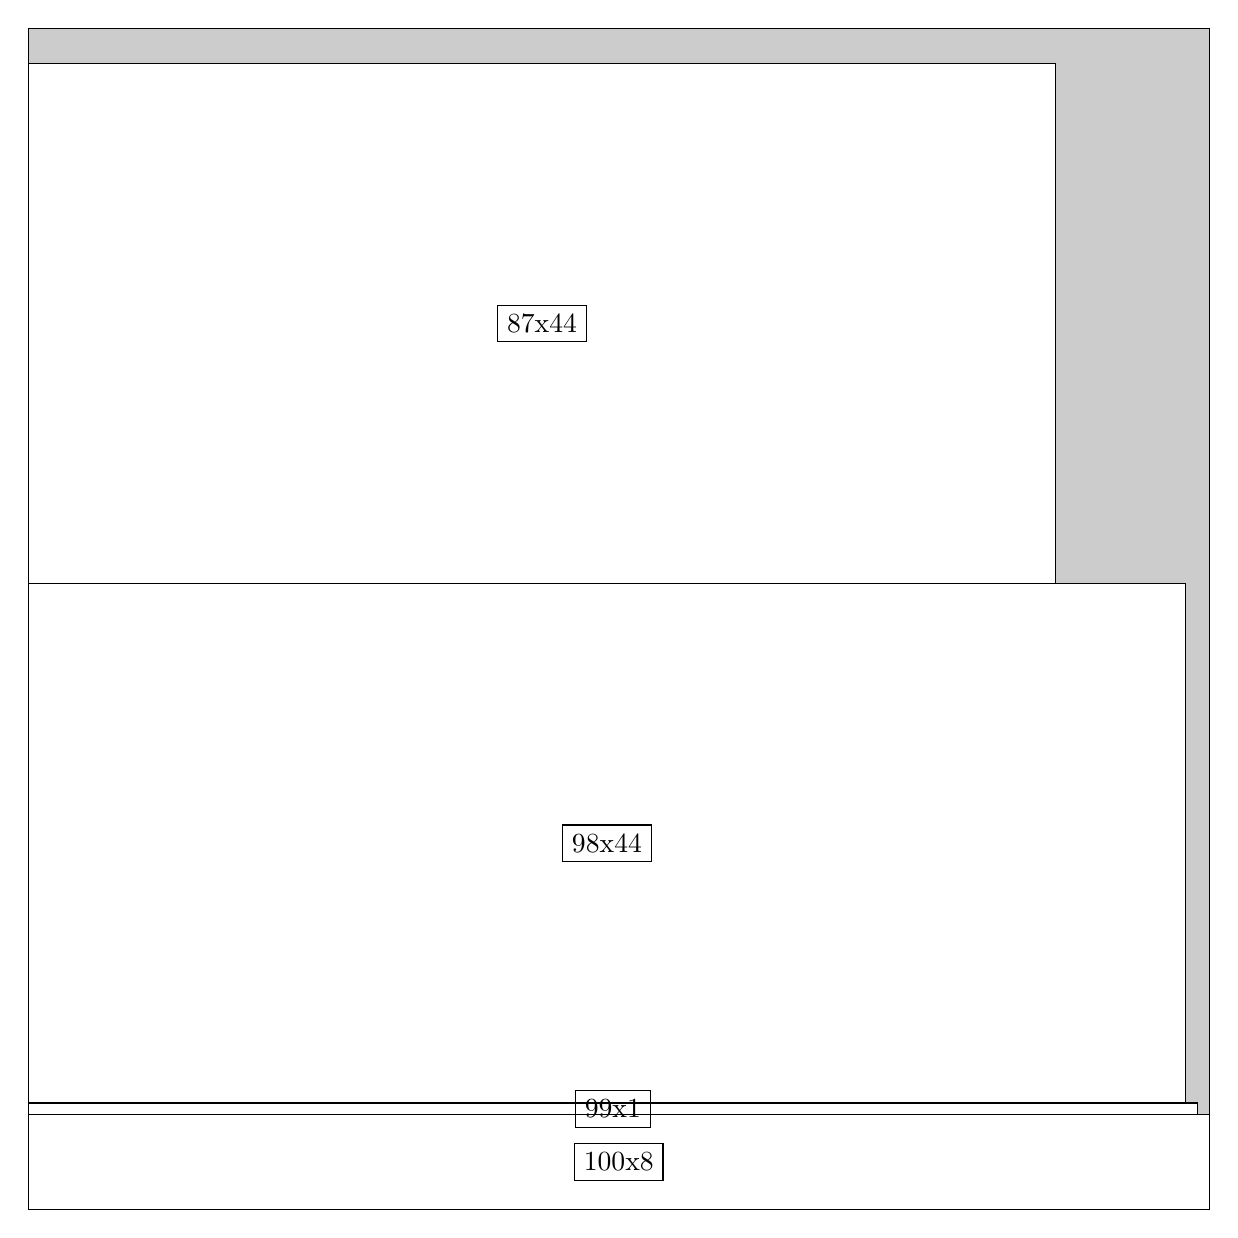
\begin{tikzpicture}[shorten >=1pt,scale=1.0,every node/.style={scale=1.0},->]
\tikzstyle{vertex}=[circle,fill=black!25,minimum size=14pt,inner sep=0pt]
\filldraw[fill=gray!40!white, draw=black] (0,0) rectangle (15.0,15.0);
\foreach \name/\x/\y/\w/\h in {98x44/0.0/1.3499999999999999/14.7/6.6,87x44/0.0/7.949999999999999/13.049999999999999/6.6,100x8/0.0/0.0/15.0/1.2,99x1/0.0/1.2/14.85/0.15}
\filldraw[fill=white!40!white, draw=black] (\x,\y) rectangle node[draw] (\name) {\name} ++(\w,\h);
\end{tikzpicture}


w =98 , h =44 , x =0 , y =9 , v =4312
\par
w =87 , h =44 , x =0 , y =53 , v =3828
\par
w =100 , h =8 , x =0 , y =0 , v =800
\par
w =99 , h =1 , x =0 , y =8 , v =99
\par
\newpage


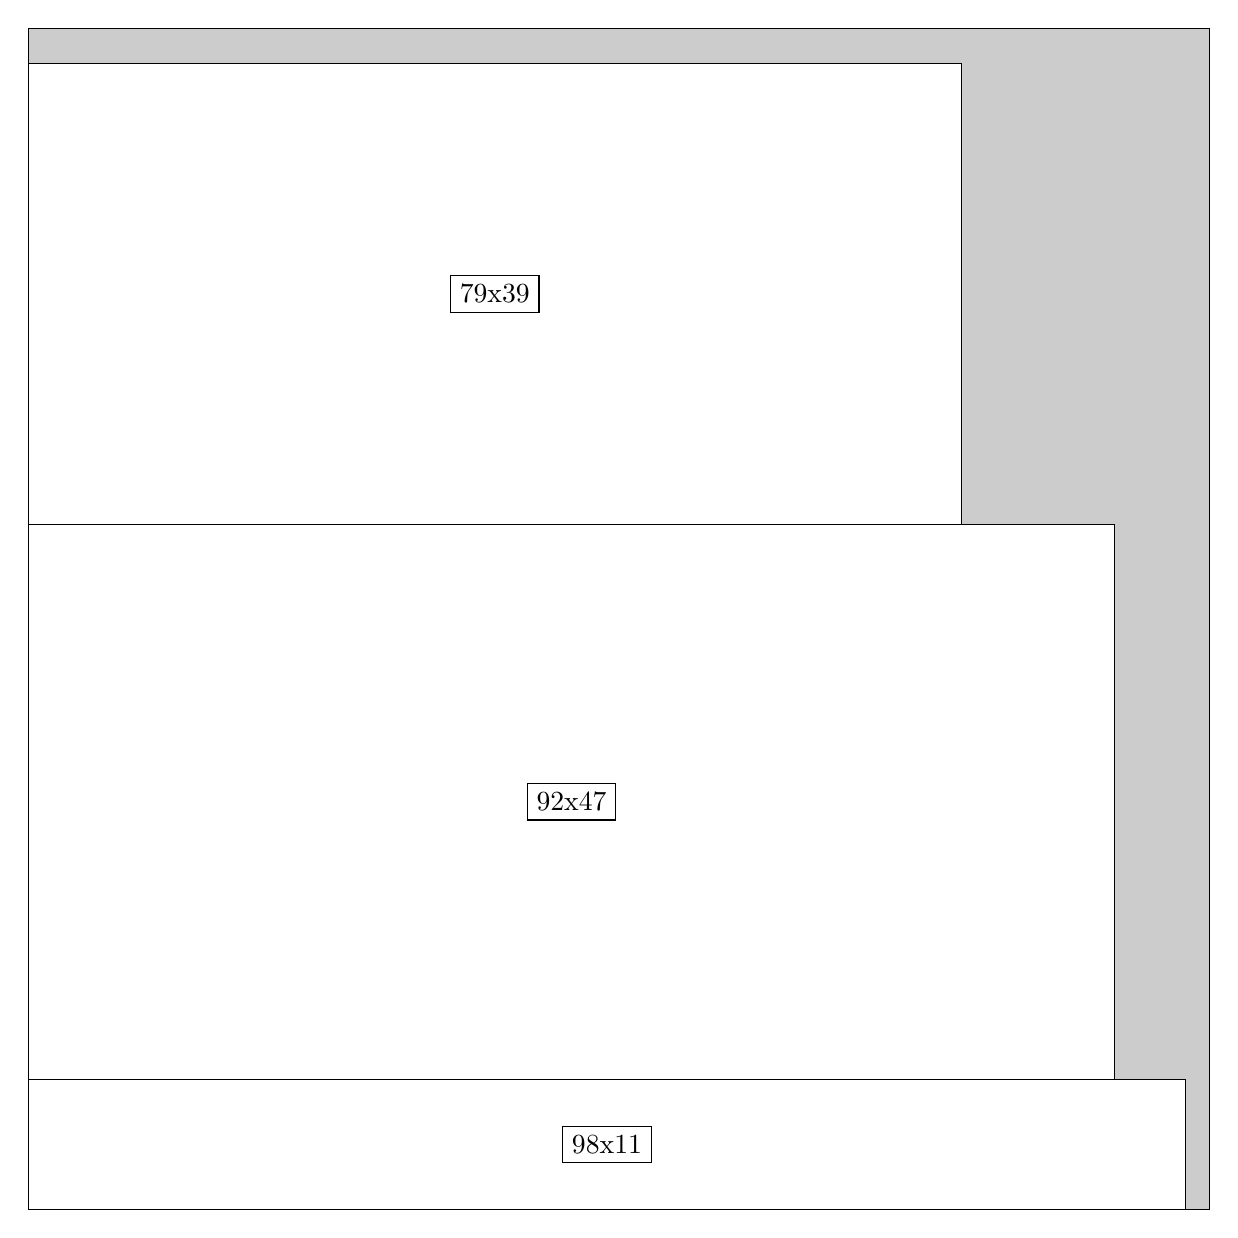
\begin{tikzpicture}[shorten >=1pt,scale=1.0,every node/.style={scale=1.0},->]
\tikzstyle{vertex}=[circle,fill=black!25,minimum size=14pt,inner sep=0pt]
\filldraw[fill=gray!40!white, draw=black] (0,0) rectangle (15.0,15.0);
\foreach \name/\x/\y/\w/\h in {92x47/0.0/1.65/13.799999999999999/7.05,79x39/0.0/8.7/11.85/5.85,98x11/0.0/0.0/14.7/1.65}
\filldraw[fill=white!40!white, draw=black] (\x,\y) rectangle node[draw] (\name) {\name} ++(\w,\h);
\end{tikzpicture}


w =92 , h =47 , x =0 , y =11 , v =4324
\par
w =79 , h =39 , x =0 , y =58 , v =3081
\par
w =98 , h =11 , x =0 , y =0 , v =1078
\par
\newpage


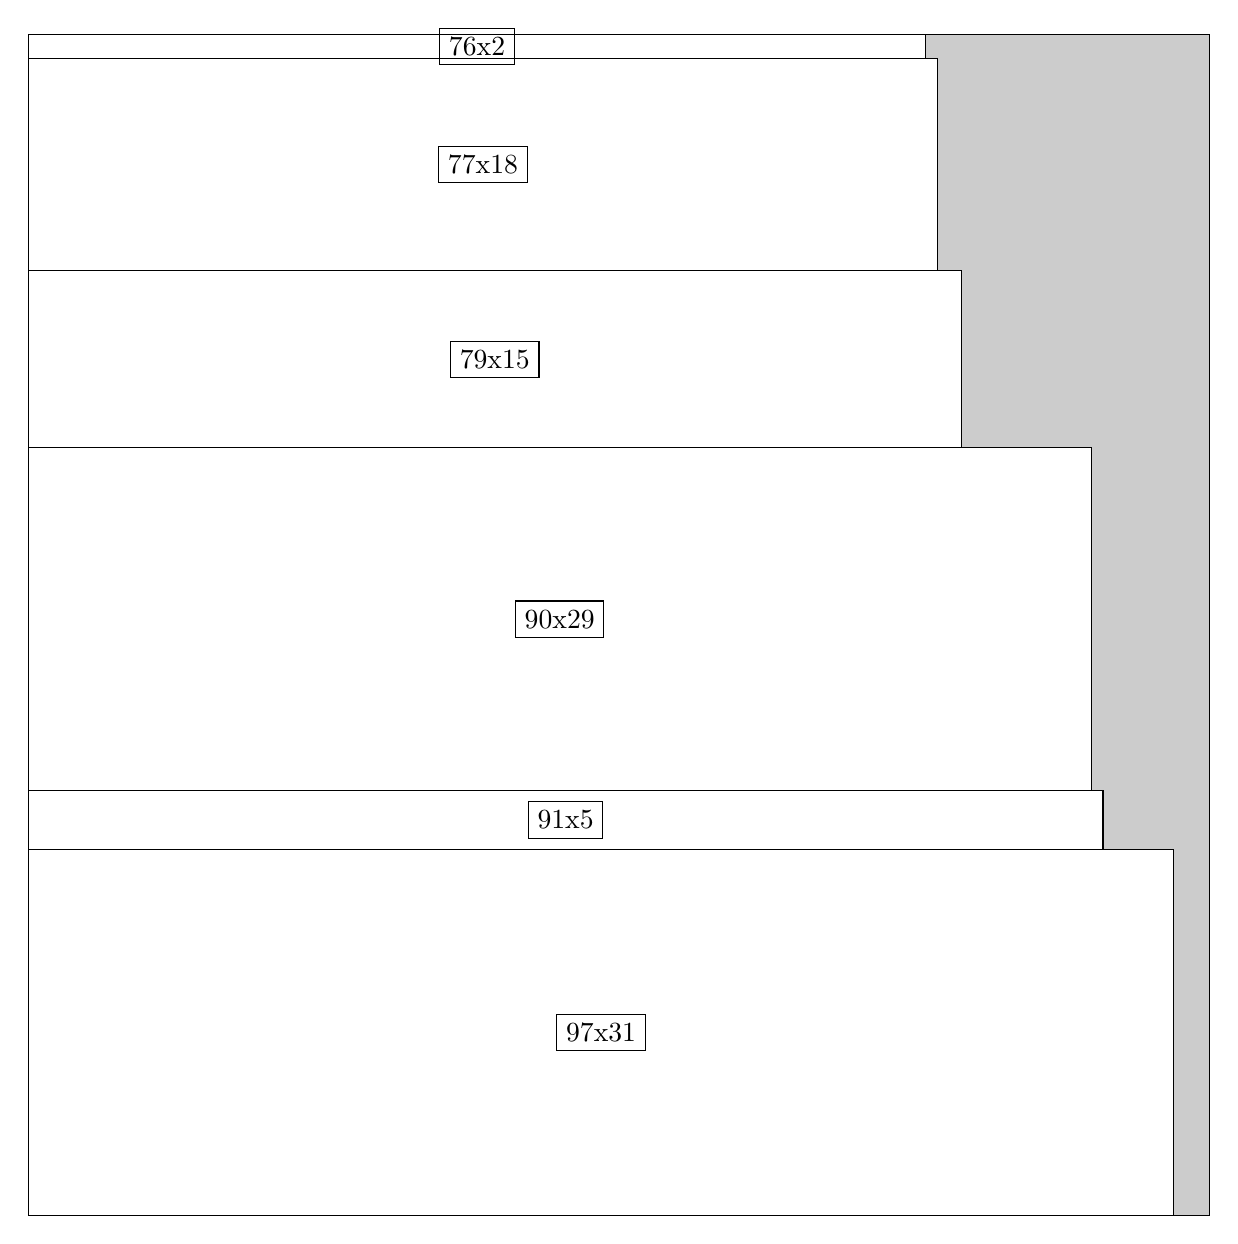
\begin{tikzpicture}[shorten >=1pt,scale=1.0,every node/.style={scale=1.0},->]
\tikzstyle{vertex}=[circle,fill=black!25,minimum size=14pt,inner sep=0pt]
\filldraw[fill=gray!40!white, draw=black] (0,0) rectangle (15.0,15.0);
\foreach \name/\x/\y/\w/\h in {79x15/0.0/9.75/11.85/2.25,97x31/0.0/0.0/14.549999999999999/4.6499999999999995,90x29/0.0/5.3999999999999995/13.5/4.35,77x18/0.0/12.0/11.549999999999999/2.6999999999999997,91x5/0.0/4.6499999999999995/13.65/0.75,76x2/0.0/14.7/11.4/0.3}
\filldraw[fill=white!40!white, draw=black] (\x,\y) rectangle node[draw] (\name) {\name} ++(\w,\h);
\end{tikzpicture}


w =79 , h =15 , x =0 , y =65 , v =1185
\par
w =97 , h =31 , x =0 , y =0 , v =3007
\par
w =90 , h =29 , x =0 , y =36 , v =2610
\par
w =77 , h =18 , x =0 , y =80 , v =1386
\par
w =91 , h =5 , x =0 , y =31 , v =455
\par
w =76 , h =2 , x =0 , y =98 , v =152
\par
\newpage


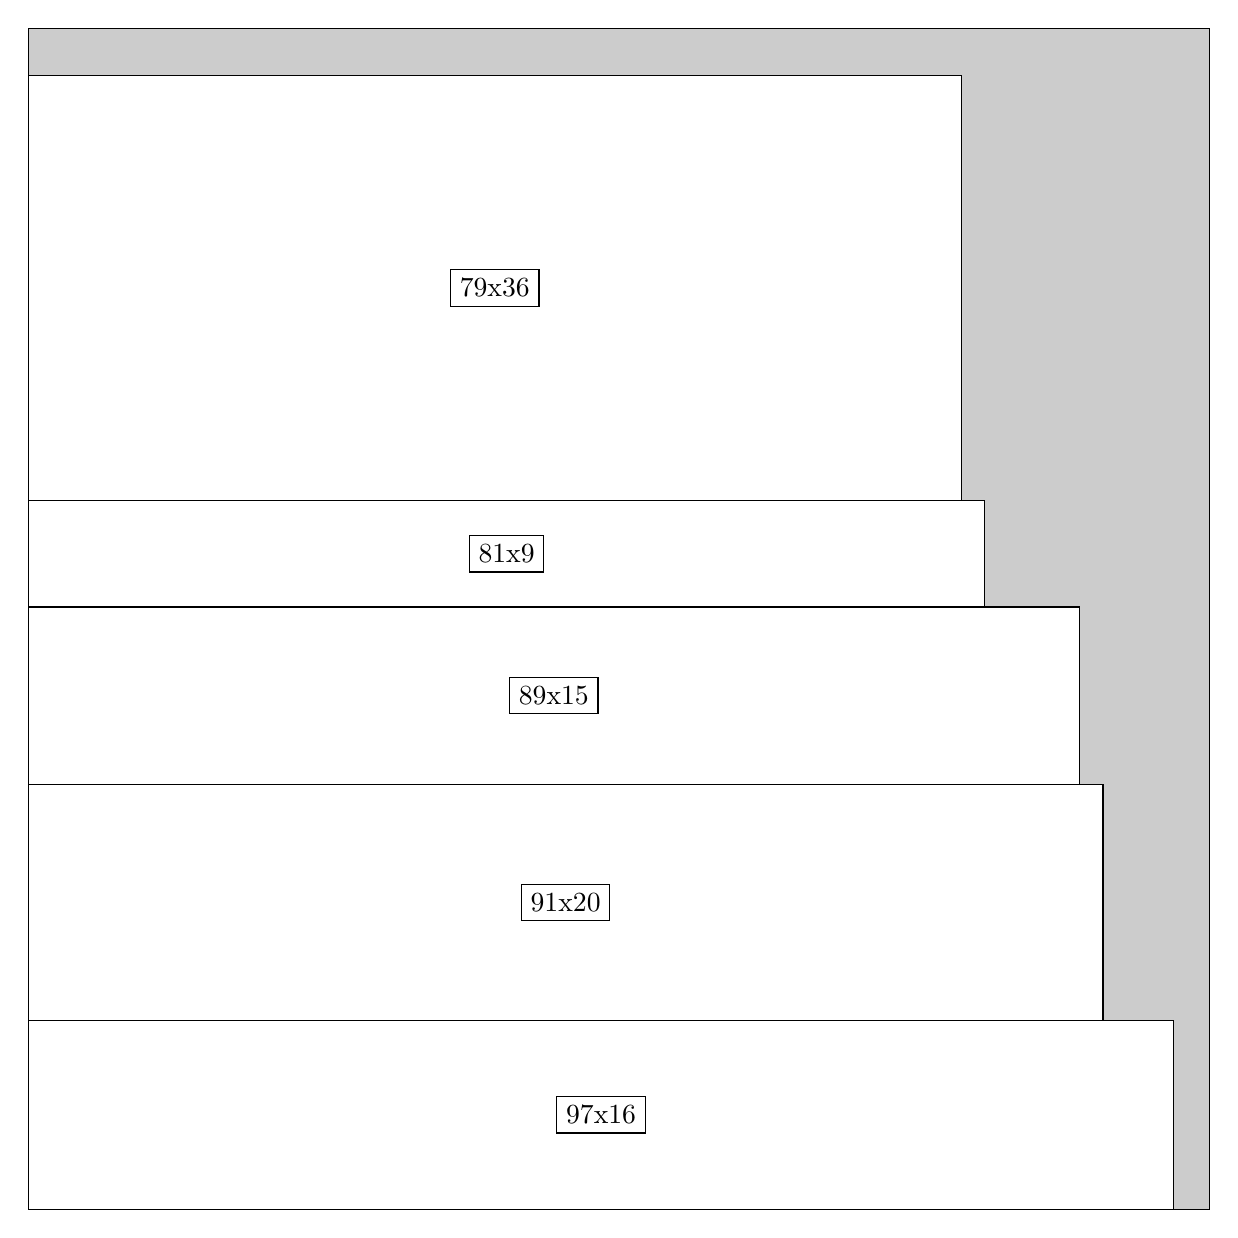
\begin{tikzpicture}[shorten >=1pt,scale=1.0,every node/.style={scale=1.0},->]
\tikzstyle{vertex}=[circle,fill=black!25,minimum size=14pt,inner sep=0pt]
\filldraw[fill=gray!40!white, draw=black] (0,0) rectangle (15.0,15.0);
\foreach \name/\x/\y/\w/\h in {79x36/0.0/9.0/11.85/5.3999999999999995,91x20/0.0/2.4/13.65/3.0,97x16/0.0/0.0/14.549999999999999/2.4,89x15/0.0/5.3999999999999995/13.35/2.25,81x9/0.0/7.6499999999999995/12.15/1.3499999999999999}
\filldraw[fill=white!40!white, draw=black] (\x,\y) rectangle node[draw] (\name) {\name} ++(\w,\h);
\end{tikzpicture}


w =79 , h =36 , x =0 , y =60 , v =2844
\par
w =91 , h =20 , x =0 , y =16 , v =1820
\par
w =97 , h =16 , x =0 , y =0 , v =1552
\par
w =89 , h =15 , x =0 , y =36 , v =1335
\par
w =81 , h =9 , x =0 , y =51 , v =729
\par
\newpage


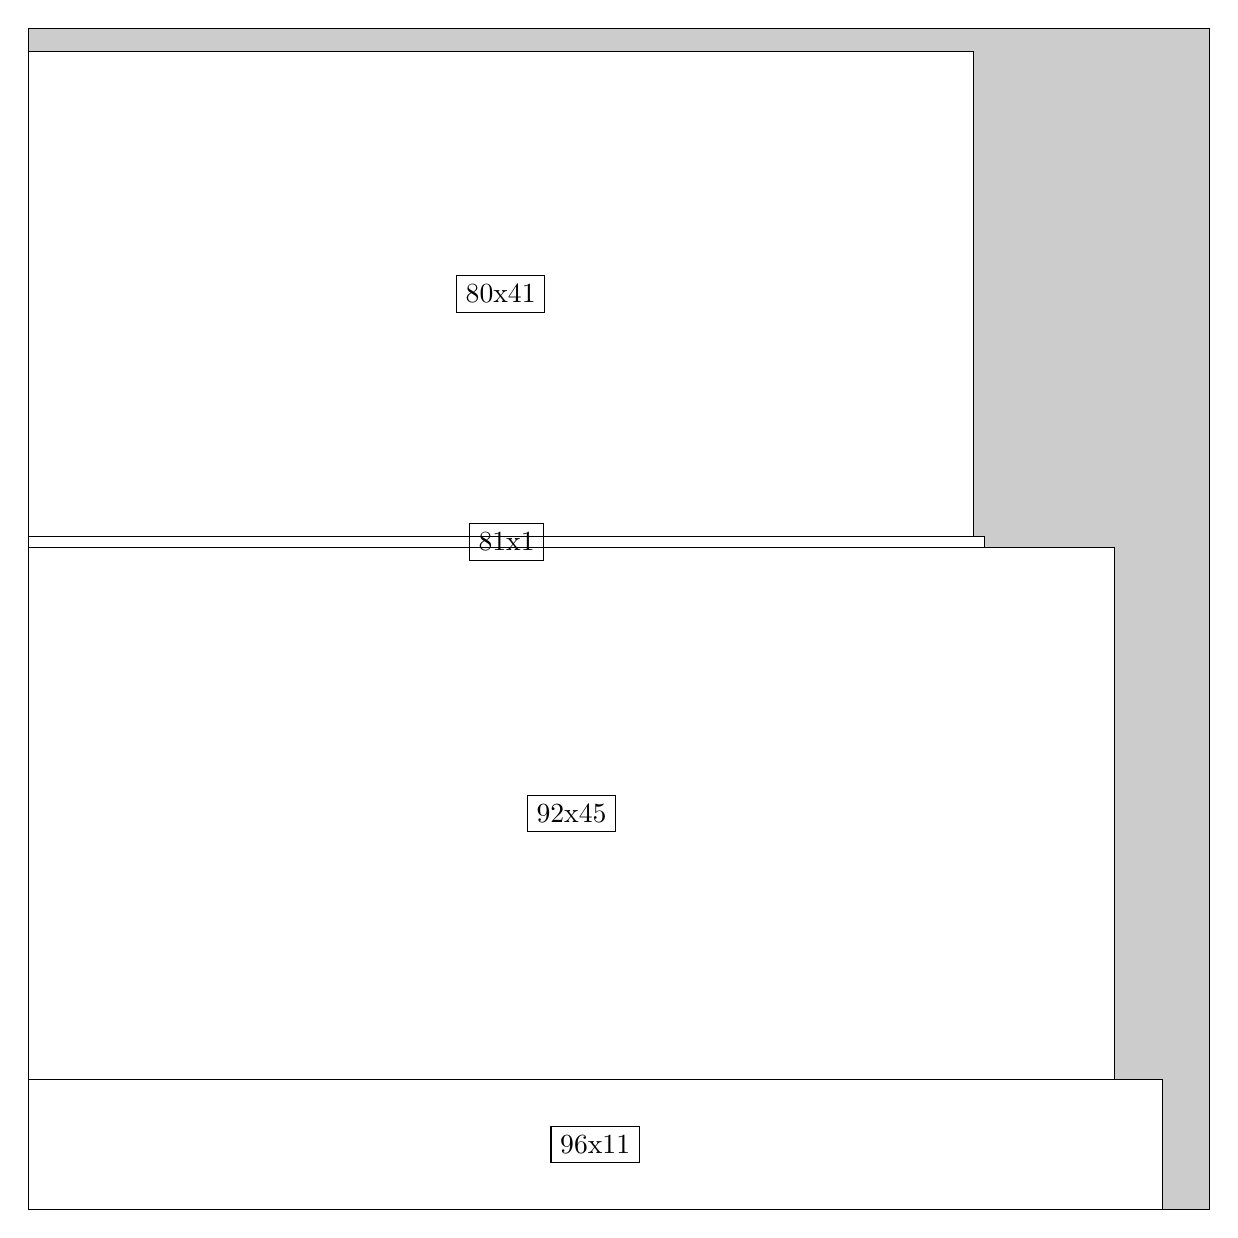
\begin{tikzpicture}[shorten >=1pt,scale=1.0,every node/.style={scale=1.0},->]
\tikzstyle{vertex}=[circle,fill=black!25,minimum size=14pt,inner sep=0pt]
\filldraw[fill=gray!40!white, draw=black] (0,0) rectangle (15.0,15.0);
\foreach \name/\x/\y/\w/\h in {92x45/0.0/1.65/13.799999999999999/6.75,80x41/0.0/8.549999999999999/12.0/6.1499999999999995,96x11/0.0/0.0/14.399999999999999/1.65,81x1/0.0/8.4/12.15/0.15}
\filldraw[fill=white!40!white, draw=black] (\x,\y) rectangle node[draw] (\name) {\name} ++(\w,\h);
\end{tikzpicture}


w =92 , h =45 , x =0 , y =11 , v =4140
\par
w =80 , h =41 , x =0 , y =57 , v =3280
\par
w =96 , h =11 , x =0 , y =0 , v =1056
\par
w =81 , h =1 , x =0 , y =56 , v =81
\par
\newpage


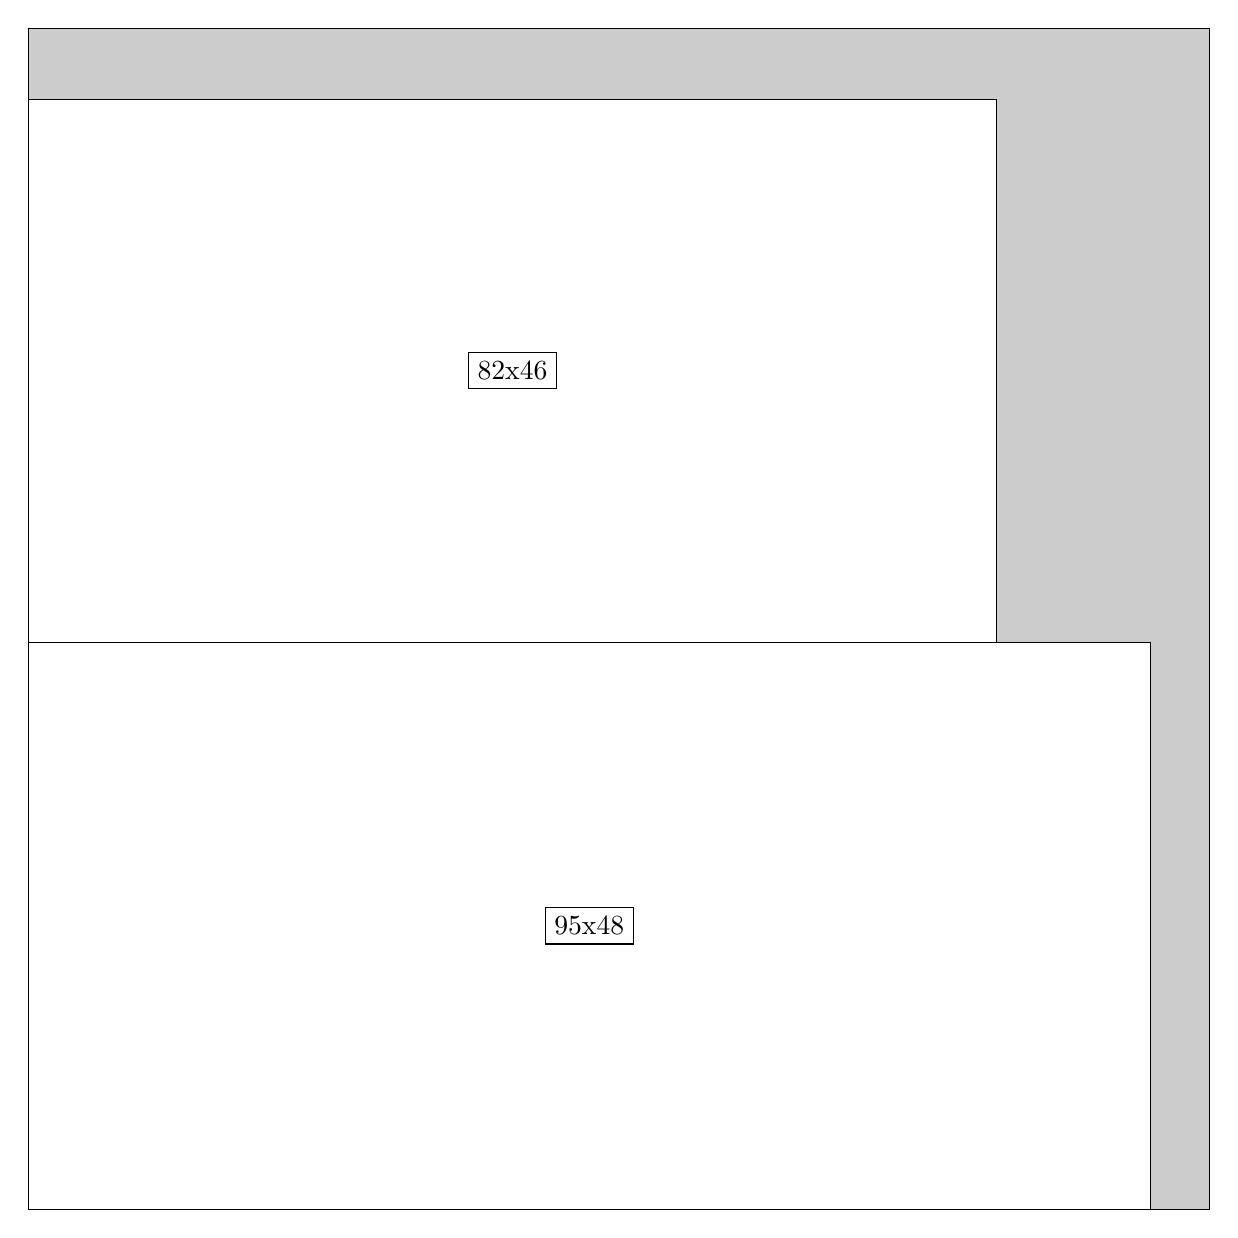
\begin{tikzpicture}[shorten >=1pt,scale=1.0,every node/.style={scale=1.0},->]
\tikzstyle{vertex}=[circle,fill=black!25,minimum size=14pt,inner sep=0pt]
\filldraw[fill=gray!40!white, draw=black] (0,0) rectangle (15.0,15.0);
\foreach \name/\x/\y/\w/\h in {95x48/0.0/0.0/14.25/7.199999999999999,82x46/0.0/7.199999999999999/12.299999999999999/6.8999999999999995}
\filldraw[fill=white!40!white, draw=black] (\x,\y) rectangle node[draw] (\name) {\name} ++(\w,\h);
\end{tikzpicture}


w =95 , h =48 , x =0 , y =0 , v =4560
\par
w =82 , h =46 , x =0 , y =48 , v =3772
\par
\newpage


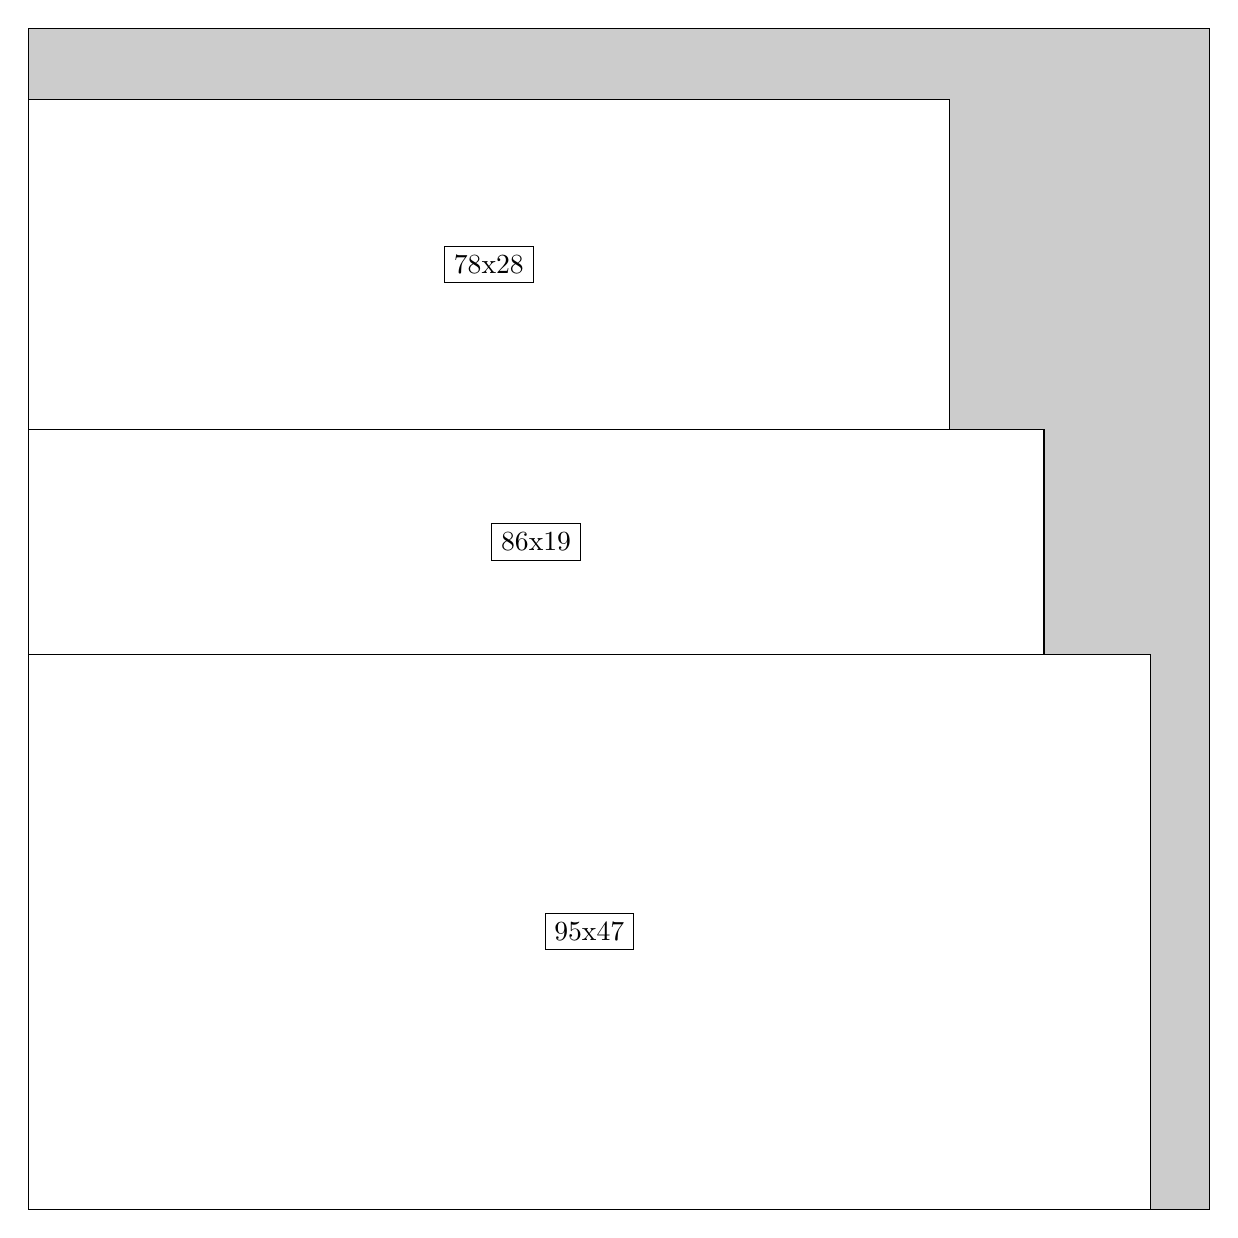
\begin{tikzpicture}[shorten >=1pt,scale=1.0,every node/.style={scale=1.0},->]
\tikzstyle{vertex}=[circle,fill=black!25,minimum size=14pt,inner sep=0pt]
\filldraw[fill=gray!40!white, draw=black] (0,0) rectangle (15.0,15.0);
\foreach \name/\x/\y/\w/\h in {95x47/0.0/0.0/14.25/7.05,78x28/0.0/9.9/11.7/4.2,86x19/0.0/7.05/12.9/2.85}
\filldraw[fill=white!40!white, draw=black] (\x,\y) rectangle node[draw] (\name) {\name} ++(\w,\h);
\end{tikzpicture}


w =95 , h =47 , x =0 , y =0 , v =4465
\par
w =78 , h =28 , x =0 , y =66 , v =2184
\par
w =86 , h =19 , x =0 , y =47 , v =1634
\par
\newpage


\end{document}